% University of Michigan Dissertation LaTeX Template for 2023
% Created by John Meluso and Shreyas Kousik
% 9 Jul 2020

% Use the University of Michigan thesis class.
\documentclass[thesis]{thesis-umich}
%%% Packages included in thesis-umich class
%\RequirePackage[margin=1in,footskip=8pt,headsep=0.4cm,headheight=\baselineskip]{geometry}
%\RequirePackage{amsmath}
%\RequirePackage{amsfonts}
%\RequirePackage{amssymb}
%\RequirePackage{graphicx}
%\RequirePackage{subcaption}
%\RequirePackage{times}
%\RequirePackage{natbib}
%\RequirePackage{verbatim}
%\RequirePackage{upquote}
%\RequirePackage{textcomp}
%\RequirePackage{setspace}
%\RequirePackage{ifthen}
%\RequirePackage{soul}
%\RequirePackage{float}
%\RequirePackage{acronym}
%\RequirePackage{makeidx}
%\RequirePackage{fancyhdr}
%\RequirePackage{multicol}

% Include your packages here by including a \usepackage{<package_name>} command.
\usepackage{blindtext} % Example package which populates the ever-popular lorem ipsum text.
\usepackage{algorithm}
\usepackage{algpseudocode}

%--- Set the font styles -----
% As of this writing, Rackham does not have strict font requirements, but they
% suggest "standard fonts" such as Times, Arial, or Times New Roman.
% In practice, they allow the default LaTeX font (Computer Modern).
% The fonts available to you depend on the typesetting engine you use, e.g.
% pdflatex (the overleaf default), xelatex, or lualatex.
% Set the font to whatever you like, as long as it's compatible with the tex
% engine you're using.
% More information from Overleaf on font selection with:
%     - pdflatex: https://www.overleaf.com/learn/latex/Font_typefaces
%     - xelatex: https://www.overleaf.com/learn/latex/XeLaTeX
% See examples below depending on your engine and uncomment the usepackage
% commands and any subsequent commands as needed.
%-------------------------------------------------------------------------------
%--- pdflatex -----
%\usepackage{times}
%\usepackage{newtxtext}
%\usepackage{newtxmath}
%-------------------------------------------------------------------------------
%--- xelatex / lualatex -----
%\usepackage{fontspec}
%\setromanfont{Times New Roman}
%\setsansfont{Arial}
%\setmonofont{Courier New}
%-------------------------------------------------------------------------------

% If you are using the alpha bibliography style, keep these next three lines in your preamble, so that the references are left-aligned; or, you can comment it out and see what happens
\makeatletter
\renewcommand{\@biblabel}[1]{[#1]\hfill}
\makeatother

% Title of the thesis
\title{Investigations into Mutation Rates and Statistical Phasing Errors}

% Author name
\author{Andrew T. Beck}

% Specify the author's legal name, if different from the preferred name.
%\legalname{Your Legal Name}

% Department
\department{Biostatistics}

% Year of completion
\year=2025

% Author email
\email{beckandy@umich.edu}

% Author ORCID iD
\orcid{0000-0002-2516-2423}

% Frontispiece
% \frontispiece{\includegraphics[width=4in]{front_materials/frontispiece.png}}

% Default style for front pages
\frontpagestyle{7} % 7 is preferred by Rackham, but should be set individually for each front page

% Dedication (the input [7] determines the style -- 7 is Rackham's preferred style)
% \hidededication{%
% \dedication[7]{\input{front_materials/dedication}}

% Acknowledgments (the input [7] determines the style -- 7 is Rackham's preferred style)
% \acknowledgments[7]{\input{front_materials/acknowledgments}}

% Preface
% \preface[7]{\input{front_materials/preface}}

% Committee
\committee{ %
Professor Sebastian Z\"{o}llner, Chair \\
Professor Veera Baladandayuthapani, Member \\
Professor Hui Jiang, Member \\
Professor Xiang Zhou, Member \\
Professor Jun Li, Cognate
}

% Chair must be entered separately for formatting reasons.
\chair{Professor Sebastian}
%\cochair{Co-chair One \& Co-chair Two}


% Definition of any acronyms used.
% To add an acronym, add an \acro{}{} command on a new line within the \acronyms{} command. For \acro, field 1 is the acronym and field 2 is the corresponding expression. For example: \acro{TLA}{Three Letter Acronym}.
\acronyms{
    \acro{NGS}{Next Generation Sequencing}
    \acro{SOA}{Some Other Acronym}
}

% Definition of any symbols used.
% To add an symbol, add an \item command with the symbol inside a [] bracket followed by explanations
\symbols{
    \item [$\alpha$] The greek letter alpha.
    \item [$\Gamma$] \blindtext
}

% Commands to hide or show lists of figures, tables, etc.
% To hide a list, change the word "show" in the command to "hide".
\hidelistoftables
\hidelistofprograms
\hidelistofappendices
\hidelistofacronyms
\hidelistofsymbols
\hidelistoffigures

% Some abstract text
%\abstract{
%\input{front_materials/abstract}
%}
%\hideabstractpagenumber

%% DOCUMENT AREA
\begin{document}

\chapter{Introduction}
\label{chpt:introduction}

The development of Next Generation Sequencing (NGS) has revolutionized the study of genetic variation, allowing for the analysis of many genomes in a fast and cost-efficient manner \citep{Bagger2024}. These developments have enabled the study of the genetic components of a vast number of heritable traits \citep{Sollis2022, Szustakowski2021}, and such results are being used to both identify and characterize biological mechanisms underlying diseases and traits \citep{Gallagher2018}, and to develop polygenic risk scores to better predict an individual's risk of developing certain diseases and better personalize medical care \citep{Lewis2020}. In addition, the generation of large numbers of genome sequences has also allowed for the study of genome diversity and evolution through the analysis of genome-wide patterns of selection, recombination and linkage disequilibrium, and mutation processes \citep{Marchi2021}.

Mutation rates are a key feature of many demographic inference tools, and as the source of all heritable genetic variation, the rates at which they occur along the genome along with the evolution of the underlying processes are themselves the focus of much investigation \citep{Carlson2018, Chintalapati2020, Gao2019, Harris2017, Moore2021, Narasimhan2017, Seplyarskiy2023, Seplyarskiy2021b, Seplyarskiy2021a, Sgurel2014}. In evaluations of mutation rate models, various genomic features have been identified as being associated with either increased or decreased rates of mutations; such features include early/late replication timing, recombination rates, methylation markers, and the nucleotide sequence context of the putative mutation site \citep{Carlson2018, Seplyarskiy2023}. In particular, \citep{Carlson2018} found that the influence of genomic features such as DNAse hypersensitive sites and GC content were associated with both increased and decreased rates of mutation, depending on both the type of mutation under consideration, and the sequence context surrounding the putative mutation site. When incorporating local sequence context in models of mutation rates, choices must be made in regards to how many neighboring positions are to be included, and to what extent interactions among neighboring nucleotides also are to be accounted for. A straighforward-way to incorporate local sequence context into mutation rate models is to consider mutation subtypes not only by the reference and alternative allele at a focal position, but also by the nucleotides at surrounding positions. By fitting separate models for each motif-mutation category, the influence of local sequence context is controlled for not only the individual effects of each included flanking position, but all orders of interaction among the nucleotides at those positions. Taking such an approach, \citep{Carlson2018} found that models which included flanking nucleotides in a $\pm 3$ window surrounding the focal position outperformed models that incorporated fewer flanking positions. However, the addition of additional flanking positions in the motif-category approach causes an exponential increase in the number of categories, and thus limits the size of local sequence context windows used in practice. \citep{Seplyarskiy2023} employed a more flexible approach by augmenting a $\pm 2$ base-pair motif-category model with independent effects for neighboring bases further up/down-stream from the focal position. This assumes that the influence of interactions among neighboring positions on rates of mutation at a focal position are contained within the $\pm 2$ base-pair window, and that the additional influence of additional neighboring positions is captured through independent parameters with no additional interactions. While it seems reasonable to assume that neighboring positions closer a focal position would exert more influence on the probability of a mutation, these assumptions have yet to have been fully explored, and it is an open question as to how far from a focal position would we expect neighboring nucleotides to have an influence on mutation rates, and to what extent and degree do interactions among neighboring sequences have influence on mutation rates.
 
In the generation of NGS data, what we observe are the genotypes at positions along the genome. However, in many applications we would like to know not only which combinations of variants an individual carries along their genomes, but also which variants traveled with each other on the same chromosomes. This requires the reconstruction of phased chromosomes, which can be performed in a number of ways. For short-read NGS data, we generally rely on two approaches: applying the laws of Mendelian inheritance to construct haplotypes when related pedigrees of individuals are sequenced, or statistical phasing methods when we do not have samples from related pedigrees. Modern statistical phasing algorithms \citep{Browning2021, Hofmeister2023, Loh2016} are able to generate highly accurate phasing results for large samples in a computationally efficient manner, but their accuracy depends largely on sample size and reference composition, and errors are generated. 

In the second chapter of this disseration,

In the third chapter of this dissertation,

In the fourth chapter of this dissertation,
% Place your additional chapters here using the \input{} command
\chapter{Evaluating the influence of local sequence context on rates of mutation}
\label{chpt:introduction}
\chapter{Deep evaluation of modern statistical phasing algorithms}
\label{chpt:phasingEval}

Modern sequencing studies have greatly increased the availability of genetic information from individuals across a wide range of ancestral backgrounds, providing a rich resource for a wide variety of analyses. Whole-genome and whole-exome sequencing (WGS/WES) studies of large cohorts has allowed for the identification of rare variants and their contributions to disease risk and trait heritability (\citep{Wainschtein2022, Wang2021}). Analyses beyond identifying variant-trait associations often require phased haplotypes, which are not directly observed in WGS or WES studies. For example, the identification of compound heterozygous events, wherein both copies of a gene contain different heterozygous variants, requires accurate phase information. Other downstream analyses, such as imputation(\citep{Howie2012,Das2016,Das2018}), demographic inference (\citep{Maples2013,Baran2012,SalterTownshend2019}), and testing for natural selection (\citep{Browning2020NS, Sabeti2002, Hanchard2006, Zhang2006}) either require or prefer phased haplotypes. Population-based phasing methods allow for the statistical inference of haplotypes in large samples of unrelated individuals. While the availability of larger samples and high quality reference panels have led to improvements in phasing accuracy, modern phasing algorithms still introduce thousands of switch errors in each phased genome \cite{Choi2018}. These errors impact downstream analyses, and therefore a comprehensive analysis of their frequency and the genomic contexts in which they occur more frequently is of considerable interest.

Previous efforts to benchmark phasing methods have relied on the availability of either trio genotyping or sequencing data, or genomes phased using a combination of multiple sequencing platforms and experimental techniques \citep{Choi2018}. While the pedigree information allows for the construction of phased haplotypes under the principles of Mendelian inheritance, switch and flip error rates estimated from trio data have been shown to be inflated due to genotyping error \citep{Browning2022}. In addition, the cost of obtaining parent-child trios often precludes their widespread use in genetic studies, whereas large samples of unrelated individuals are readily available \citep{ByrskaBishop2022}. A phasing evaluation which leveraged such a large sample would allow for a more detailed characterization of phasing errors across chromosomes. However, the absence of gold-standard haplotypes in this setting does not allow for a direct evaluation of phasing methods. Thus previous efforts to benchmark phasing methods using these large samples of unrelated individuals have relied on imputation quality as a downstream metric of phasing quality \citep{Stahl2021, DeMarino2022}. Imputation accuracy is a reflection of the underlying phasing quality and thus allows for a comparison across methods, but it does not allow for a detailed characterization of the genomic context in which phasing errors occur as the number and location of phasing errors are unknown. 

Here we evaluate phasing algorithms directly by constructing synthetic diploids with known phase by sampling male X chromosomes from unrelated samples in the 1kGP 30x high-coverage whole genomes data set. Each synthetic diploid consists of two male X chromosomes sampled from the 2,504 phase 3 1kGP subjects. 200 synthetic diploids are generated for each of the five 1kGP super populations for a total of 1000 synthetic diploids. Each synthetic diploid is then individually phased with three modern statistical phasing methods (Beagle 5.4, Eagle 2.4, SHAPEIT5), utilizing a reference panel consisting of the 2,502 1kGP phase 3 samples who were not used to construct the synthetic diploid. The reconstructed haplotypes are then compared to the original X chromosomes to identify the location of phasing errors. In addition, we re-phase the automsomes of 602 children for which sequences from both the mother and father are available from the expanded 1kGP sample. For each child, we phase their autosomes using the 2,504 phase III samples as the reference panel, removing any member of the trio who are part of the phase III sample. We compare the population-reference phased results to the pedigree-adjusted phase to identify phasing errors. 

We classify errors into one of two categories: switches, in which the phase of a variant is incorrect with respect to the preceding variant but is correct with respect to subsequent variants; and flips, in which a single variant is incorrectly phased with respect to its neighboring variants. Without this distinction, flips would be double-counted as consecutive switch errors. With these distinctions, we compute both switch error rates:

\begin{equation}
    \textrm{SER}(i, m) = \frac{\sum_j^{n_i} s(i, j)}{n_i}
\end{equation}

and flip error rates:

\begin{equation}
    \textrm{FER}(i, m) = \frac{\sum_j^{n_i} f(i, m, j)}{n_i}
\end{equation}

where $i$ indexes the sample, $m$ indexes the method, $n_i$ denotes the number of heterozygous positions in sample $i$, and $s$ and $f$ are indicators equal to 1 if a switch or a flip, respectively, are observed at a given position for the method's inferred phase of sample $i$.

\begin{figure}
    \centering
    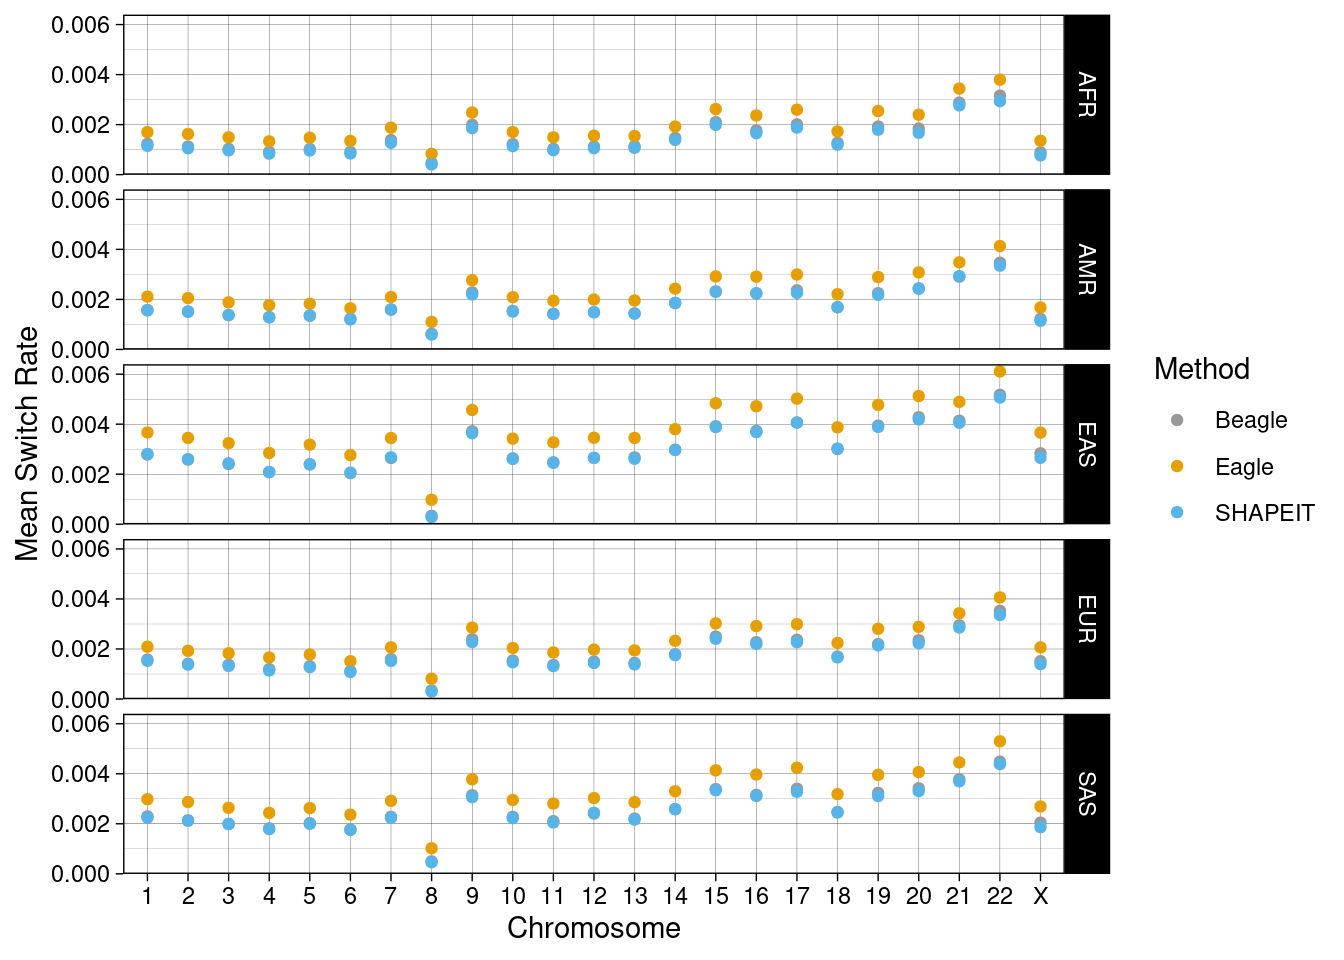
\includegraphics[scale=0.80]{chapters/figures/switch_error_rates_all.png}
    \caption{Average switch error rates by population across all autosomes and chromosome X. While rates vary by chromosome, the ranking of methods is consistent, with Eagle having higer switch error rates than Beagle and SHAPEIT.}
    \label{fig:switch_err}
\end{figure}

In addition to ranking methods by flip and switch error rates, we also evaluate the overlap of errors across methods. Additionally, we assess the distributions of error rates across the chromosomes and correlated these rates by genomic features such as recombination rates, minor allele frequencies, and GC content.
\chapter{Meta-phasing: methods for generating consensus phase from multiple algorithms}
\label{chpt:metaphase}

In chapter \ref{chpt:phasingEval} we evaluated the distribution of errors generated by three phasing algorithms. One way in which we could aggregate the results for each sample across the three methods would be to take a consensus voting approach, in which the phase at each heterozygous position would be that in which at least two methods were in agreement. Similar to \citep{AlBkhetan2020}, we describe the consensus vote approach in \ref{alg:cp}:

\begin{algorithm}
\caption{Consensus Phase Algorithm}\label{alg:cp}
\begin{algorithmic}
\State \textbf{Input}:  $\{h_1, h_2, h_3\} - \textrm{phasing estimates, } h_j \in \{0,1\}^p$
\State \textbf{Output: } \textit{cons} $\in \{0,1\}^p$
\For{$i = 0, \ldots, p$}
\State $cons[i] \gets majority\_vote(h_1[i], h_2[i], h_3[i])$
\For{$j = 1, 2, 3$}
\If{$h_j[i] \ne cons[i]$}
\State $h_j[i:p] = complement(h_j[i:p])$
\EndIf
\EndFor
\EndFor
\end{algorithmic}
\end{algorithm}

\begin{figure}
    \centering
    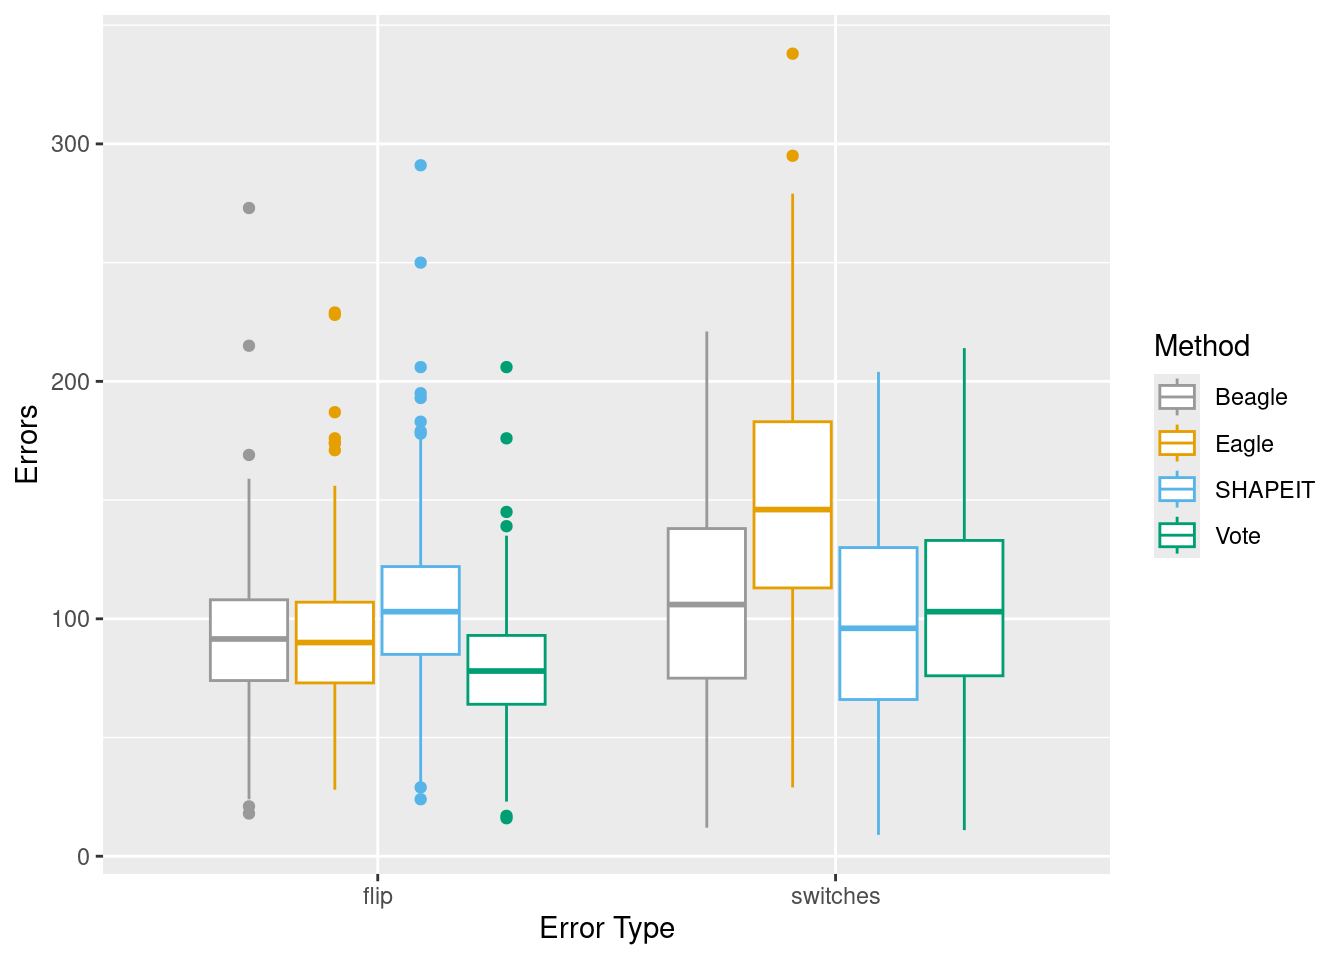
\includegraphics[scale=0.90]{chapters/figures/vote_results.png}
    \caption{Switch and flip error rate distributions over 1000 synthetic diploids by phasing method. While we generally see lower flip rates from the consensus vote approach, we don't see much of an improvement for switch error rates.}
    \label{fig:vote}
\end{figure}

When we apply the consensus vote approach to our X chromosome synthetic diploids, we see a modest improvement in flip error rates, but we don't see an improvement in switch error rates (figure \ref{fig:vote}). This is unsurprising given the extent to which we observe errors being shared across methods for each individual. In this chapter we aim to improve on the consensus vote approach by exploring alternative ways to combine results from multiple phasing algorithms. 

In the first phase of the project, we will explore error models individual phasing results. Given the sequential nature of chromosomes and how their phase can be represented as a binary vector, we will first explore models of the form seen in equation \ref{eq:phase_error}:

\begin{equation}
\label{eq:phase_error}
    e_{i,j} = \Pr(\textrm{error at position } i \textrm{, sample } j) = f(i, j) 
\end{equation}

where $f$ represents a generic class of functions that returns a probability of an error occurring at a position given some yet to be defined set of features. This set of features likely will include information on the genomic context at the position, such as average recombination rates in regions around that position in the chromosome. Additionally, we will consider ways to incorporate the sequential nature of chromosomes in these models, sharing information across neighboring heterozygous positions which might also be informative to the probability of a switch occuring at a position.

For the task of meta-phasing, we will first consider hidden markov models (HMMs), were we observe the inferred phase from multiple algorithms at each heterozygous position. We can represent these as a single binary vector where we track where each algorithm decides to place the non-reference allele realtive to the chromosome with the non-reference allele at the first heterozygous position 
(i.e., $h \in \{0,1\}^p$, $h[1] = 1$).
For the unobserved latent variable at each position, we have several options to consider, the most obvious of which is the true underlying phase at the position. In this model, the transition probabilities would then be the probability of observing either the reference or alternative allele on the true phased chromosome at the next position given the phase at the current position, and the emission probabilities would reflect whether or not each algorithm was inferring the correct phase given the true underlying state.

Another option for the hidden latent state in an HMM is to attach an indicator for each algorithm representing whether or not at the position the algorithm is placing reference and alternative alleles onto the right chromosome (equivalently, we can consider only the chromosome with the alterative allele at the first heterozygous position, in which case the indicator reflect whether the algorithm is placing the correct variant on this one chromosome). Transition probabilities from above would then be augmented with switch rates for each algorithm, while emission probabilities would either be 0 or 1, depending on the true phase at the position and the error status of the method.

% Appendices
%\appendix
%\input{appendices/example_appendix_01}
%\input{appendices/example_appendix_02}

\bibliographystyle{plain2.bst}

% Give this command the relative path to the .bib file.
\bibliography{references.bib}

\end{document}
